\section{Modelling Market Efficiency}
\label{sec:market_efficiency}

In this section, we will introduce the $Beta\_SSE$ estimate, which is our proposed measure of market inefficiency based on the unbiasedness regressions framework. It represents the level of
market under- or over-reaction at a point in time.

\subsection{Unbiasedness Regressions}

\noindent The unbiasedness regression is a simple OLS regression of the cumulative logarithmic return of the asset over a normalized window of time $\mathrm{SP500}_{[0, T]}$, on a subset of the
logarithmic cumulative returns, $\mathrm{SP500}_{[0, t]}$, where $t \leq T$, and $t$ is the number of months from the beginning of the window.
 \footnote{$\mathrm{SP500}_{[0, 1]}$ is the matrix of returns of the SP500 from January 1950 to February 1950, February 1950 to March 1950, \dots, August 2024 to September 2024, September 2024 to October 2024.\newline
$\mathrm{SP500}_{[0, 2]}$ would be the matrix of cumulative returns from January 1950 to March 1950, February 1950 to April 1950, \dots August 2024 to October 2024, and so on for the entire dataset.}

\begin{equation}
    \begin{aligned}
        \mathrm{SP500}_{[0, T]} &= \alpha_t + \beta_t \mathrm{SP500}_{[0, t]} + \epsilon_{t}, \hfill \text{   where } 0 \leq t \leq T.
    \end{aligned}
\end{equation}

\noindent For an illustrative example, let $T = 36$, so that the window $[0, T]$ represents a 3-year period, and let us look at the returns of the SP500.

\noindent For $t=1$, the regression is of the form:
\begin{equation}
    \mathrm{SP500}_{[0, 36]} = \alpha + \beta \mathrm{SP500}_{[0, 1]} + \epsilon
\end{equation}

\noindent From this regression we extract the coefficient $\beta$ and the $R^2$ value.
The regression is repeated for each partial return window $t=2, t=3, ..., t=36$, and the coefficients $\beta$ are plotted against $t$, the depth of the cumulative return window.
We plot the $\beta$ coefficients against $t$ to get a sense of the market's ability to process information over time (Figure~\ref{fig:sp_500_unbiasedness}). The $\alpha_t$ intercept
 accounts for any time-varying risk premia.

\begin{figure}[h!]
    \centering
    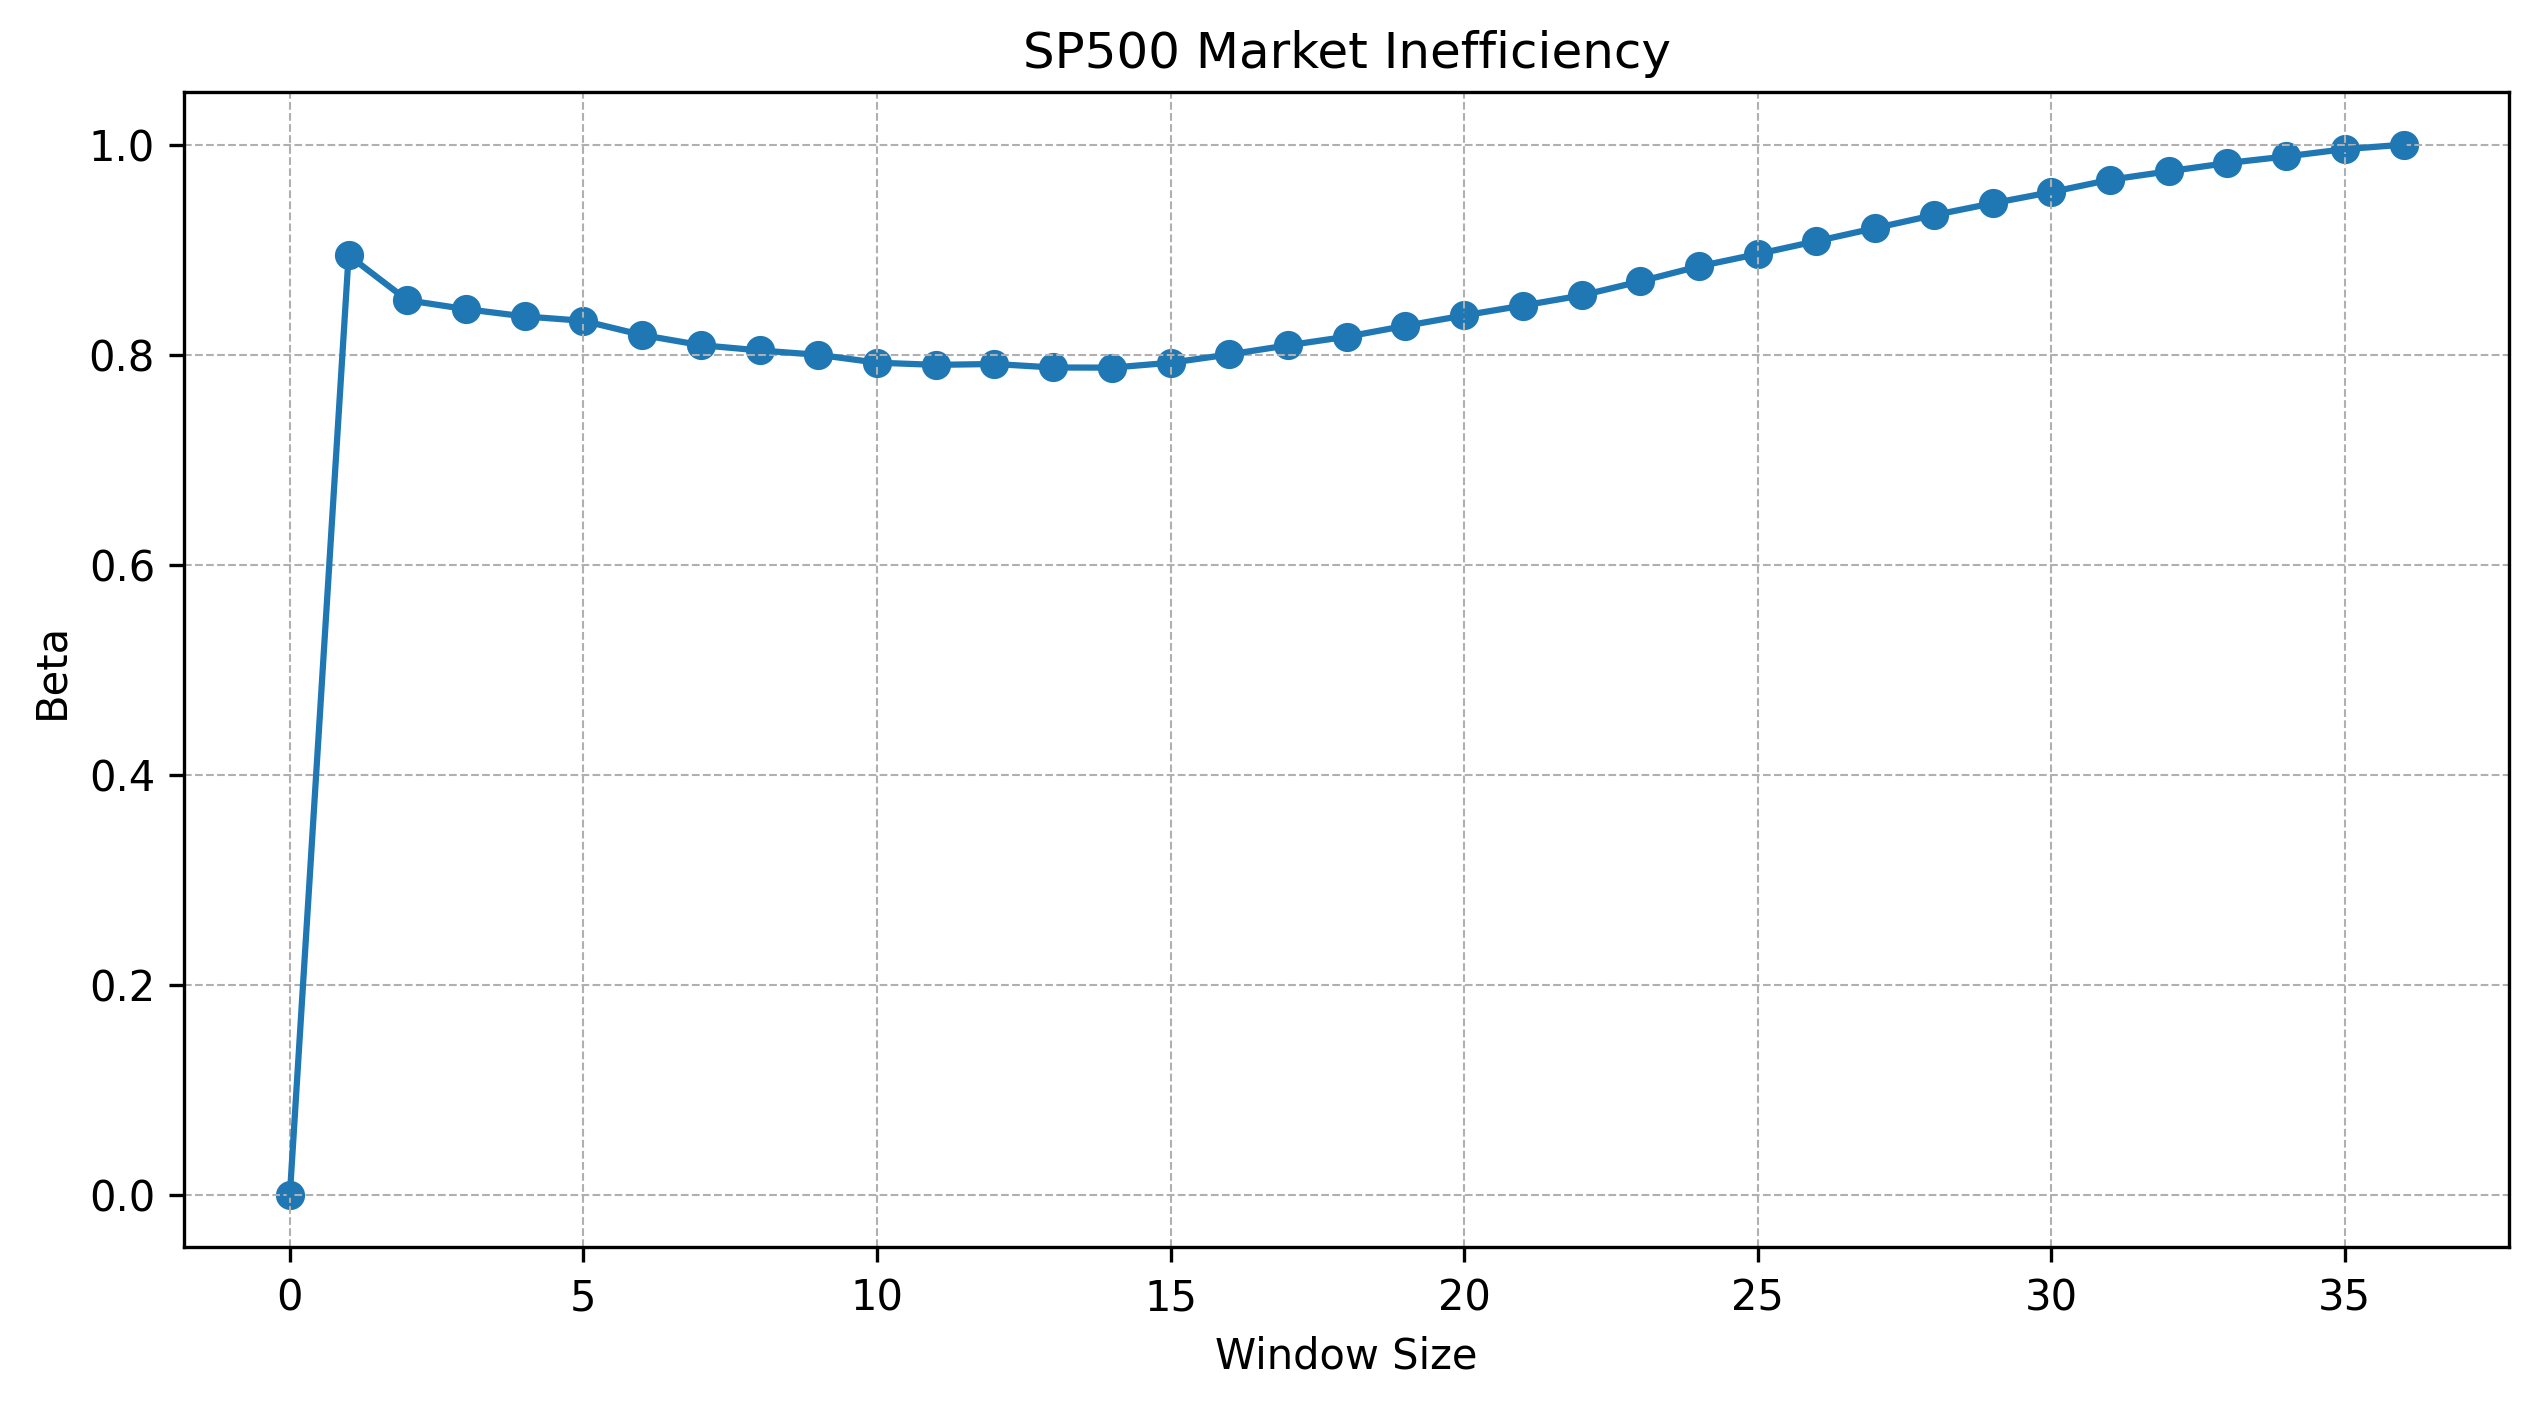
\includegraphics[width=1\textwidth]{../figs/SP500 Market Inefficiency.png}
    \caption{An unbiasedness regression on the SP500 (1950 - 2024) showing the market's tendency to overreact.}
    \label{fig:sp_500_unbiasedness}
\end{figure}

$\beta_t = 1$ for all $t$ when log prices move efficiently, following a random walk. When 
$\beta_t = 1$ the partial returns from $0$ to $t$ provide a forecast of the return from $t$ to $T$ that is as efficient as possible 
and does not need to be amplified or dampened \citep{mincer_zarnowitz_1969}. 
 If $\beta_t < 1$, the partial return is dampened in the total returns, therefore there was a temporary component in prices which decays representing an “overreaction” \citep{barclay_hendershott_2003}.
Conversely, if $\beta_t > 1$, the partial return is amplified in the total return, suggesting the market had improperly processed the information relevant in pricing the T sized window, and has underreacted.

In this paper we will be focusing on the $\beta_t$ coefficient. 
We now have the foundation to construct a score for market efficiency.

\subsection{$Beta\_SSE$ Score}

\begin{figure}[h!]
    \centering
    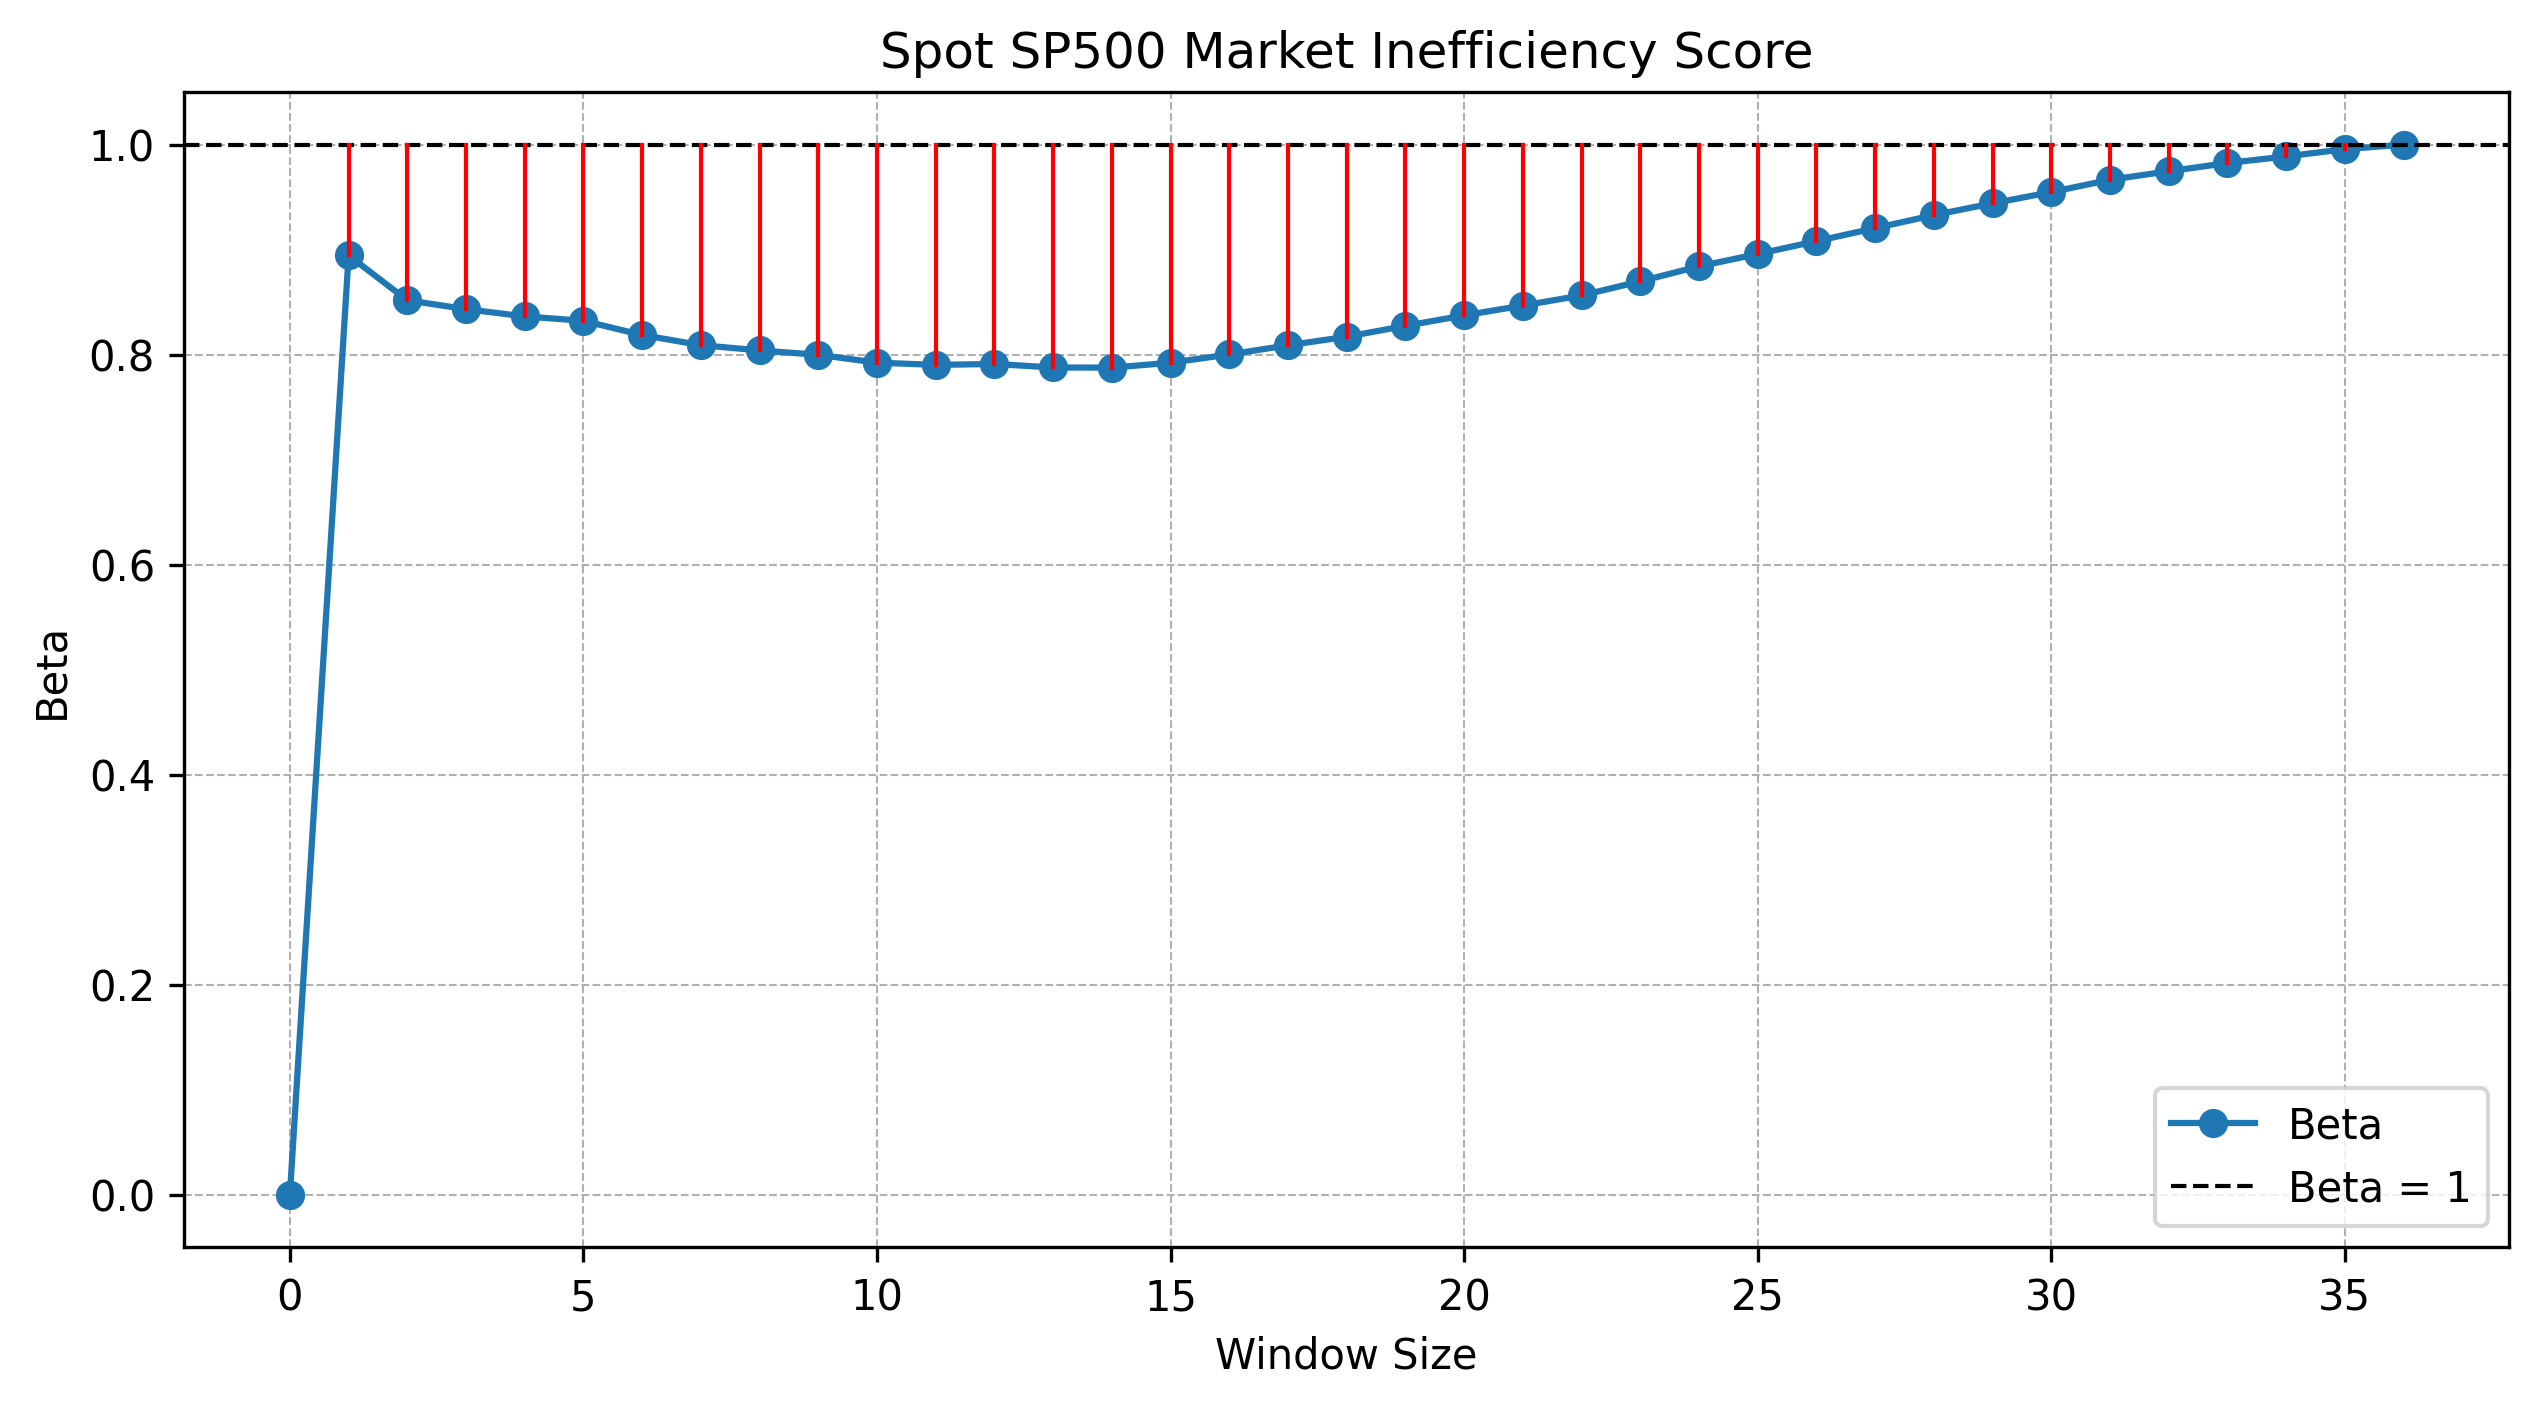
\includegraphics[width=1\textwidth]{../figs/Spot SP500 Market Inefficiency Score.png}
    \caption{A single $Beta\_SSE$ score visualization for the SP500 (1950 - 2024). The $Beta\_SSE$ score is a measure of market efficiency at a point in time, and is the sum of 
    the squares of the red distances. To construct a time series of the $Beta\_SSE$ score, we run these regressions for shingled five-year windows and plot their scores.}
    \label{fig:sp_500_unbiasedness_sse}
\end{figure}

We have established the unbiasedness regression infrastructure, and that a $\beta_t < 1$ indicates overreaction, a $\beta_t > 1$ indicates underreaction, and $\beta_t = 1$ indicates efficiency.
To construct a score that measures the level of market inefficiency at a point in time, we have to create a spot representation of the $\beta_t$ graph for a time period.

We define the $Beta\_SSE$ score as the sum of the squared differences between $\beta_t$ and the horizontal line at $\beta = 1$, for all $t$ in the window (Equation~\ref{eq:beta_sse}).
Since a $\beta_t = 1$ indicates efficiency, the $Beta\_SSE$ score will be lower when the market is more efficient and larger when the market is less efficient, whether by under- or over-reaction.
We provide a visual representation of the $Beta\_SSE$ score for the S\&P 500 over our entire data window in Figure~\ref{fig:sp_500_unbiasedness_sse}.

To construct a time series of these scores, we split our entire period of S\&P 500 returns in shingled 5-year windows. Each window is 5 years long, and the window is moved forward by 1 month at a time.
We run the same sequence of unbiasedness regressions as we did for the entire period in Figure~\ref{fig:sp_500_unbiasedness}, however on each window independently, and calculate the $Beta\_SSE$ score for each window.
So $Beta\_SSE_t$ is constructed from the unbiasedness regressions on windows of the SP500 returns from $t-60$ to $t$, where t represents a month-year.
 Note that our unbiasedness regressions extend out to $t+36$, so $Beta\_SSE_t$ score isn't tradable at time $t$ but at time $t+36$.
\footnote{Consider the rolling window [January 2000, January 2005], the observation starting at January 2005 ($t=0$ on January 2005) requires the window of returns from January 2005 to January 2008 to make $\mathrm{SP500}_{[0, 36]}$.}
This is by design, a measure of market inefficiency at a time $t$ is to be representative of the market's ability to price the $T$ months ahead.

$Beta\_SSE_t$ is calculated as follows:

\begin{equation}
    \begin{aligned}
        Beta\_SSE_t &= \sum_{i=0}^{36} (\beta_{t,i} - 1)^2
    \end{aligned}
\end{equation}
\label{eq:beta_sse}

Where $\beta_{t,i}$ is the $\beta$ coefficient from the unbiasedness regression from a 
window starting on the date $t$, at the $i$th depth of the unbiasedness window.

\subsection{Justification of Model}
Consider \citet{fama_EMH}'s definition of informational market efficiency. The market is efficient if prices at every moment incorporate all available information about future values rationally and instantaneously.
If we have a window of cumulative returns, and the market has efficiently incorporated information, and is sophisticated enough to appropriately discount future returns, we would expect cumulative returns to 
grow linearly as information comes in and aligns to the market expectation. This is the case presented when $\beta_t = 1$. 
If the market receives information during a window that does not align with expectations, we would expect the partial returns up to that point to be dampened or amplified in the total returns.
Events that would cause this are shocks such as earnings surprise, or other information that undermines the information
consumed by the market by that point. \citet{fama_EMH}'s example of potential inefficiency, that prices typically rise or fall on the release of insider information, is picked up by this framework.
It is an inefficiency, because information that was known by some participants, but not all, was not properly priced in. The market will adjust to this new information but, the price up to that point was not efficient. These are the cases when $\beta_t \neq 1$, which often spikes as these inefficiencies are shocks.
Since we are summing the squared differences, we are penalizing the market for not being efficient by under- or over-reaction, and the $Beta\_SSE$ score is an 
appropriate measure of relative market inefficiency. It does not differentiate between known possible shocks such as earnings seasons, and unprecedented shocks or black swan events, so we do see spikes of inefficiency. But, by definition of market 
efficiency we would expect it to revert to a low mean, and drift downwards over time as the market becomes increasingly better at pricing in information and less prone to surprise.
An in-depth exploration of the $Beta\_SSE$ score's properties and its relationship to market efficiency can be found in the Appendix~\ref{sec:appendix}, where we 
provide idealized results from simulations of efficient and inefficient markets.